%% 
%% Copyright 2007-2019 Elsevier Ltd
%% 
%% This file is part of the 'Elsarticle Bundle'.
%% ---------------------------------------------
%% 
%% It may be distributed under the conditions of the LaTeX Project Public
%% License, either version 1.2 of this license or (at your option) any
%% later version.  The latest version of this license is in
%%    http://www.latex-project.org/lppl.txt
%% and version 1.2 or later is part of all distributions of LaTeX
%% version 1999/12/01 or later.
%% 
%% The list of all files belonging to the 'Elsarticle Bundle' is
%% given in the file `manifest.txt'.
%% 
%% Template article for Elsevier's document class `elsarticle'
%% with harvard style bibliographic references

%\documentclass[preprint,12pt,authoryear]{elsarticle}

%% Use the option review to obtain double line spacing
\documentclass[authoryear,preprint,review,12pt]{elsarticle}

%% Use the options 1p,twocolumn; 3p; 3p,twocolumn; 5p; or 5p,twocolumn
%% for a journal layout:
%% \documentclass[final,1p,times,authoryear]{elsarticle}
%% \documentclass[final,1p,times,twocolumn,authoryear]{elsarticle}
%% \documentclass[final,3p,times,authoryear]{elsarticle}
%% \documentclass[final,3p,times,twocolumn,authoryear]{elsarticle}
%% \documentclass[final,5p,times,authoryear]{elsarticle}
%% \documentclass[final,5p,times,twocolumn,authoryear]{elsarticle}

%% For including figures, graphicx.sty has been loaded in
%% elsarticle.cls. If you prefer to use the old commands
%% please give \usepackage{epsfig}

%% The amssymb package provides various useful mathematical symbols
\usepackage{amssymb}
%% The amsthm package provides extended theorem environments
%% \usepackage{amsthm}

\usepackage{siunitx}  % for degree celsius
\usepackage{multirow} % for the table
\usepackage{booktabs} % fot toprule, midrule
\usepackage{longtable}

\usepackage{color,soul} % highlight 

% for track changes in revision version, comment this one if want the final version
%\usepackage{changes}
%\usepackage[final]{changes}

\usepackage{hyperref} %for breaking long url

%% The lineno packages adds line numbers. Start line numbering with
%% \begin{linenumbers}, end it with \end{linenumbers}. Or switch it on
%% for the whole article with \linenumbers.
%% \usepackage{lineno}

\usepackage{lineno}
\linenumbers

\journal{Remote Sensing of Environment}

\begin{document}

\begin{frontmatter}

%% Title, authors and addresses

%% use the tnoteref command within \title for footnotes;
%% use the tnotetext command for theassociated footnote;
%% use the fnref command within \author or \address for footnotes;
%% use the fntext command for theassociated footnote;
%% use the corref command within \author for corresponding author footnotes;
%% use the cortext command for theassociated footnote;
%% use the ead command for the email address,
%% and the form \ead[url] for the home page:
%% \title{Title\tnoteref{label1}}
%% \tnotetext[label1]{}
%% \author{Name\corref{cor1}\fnref{label2}}
%% \ead{email address}
%% \ead[url]{home page}
%% \fntext[label2]{}
%% \cortext[cor1]{}
%% \address{Address\fnref{label3}}
%% \fntext[label3]{}

%\ead{huanglingcao@link.cuhk.edu.hk}

\title{Automatically quantifying evolution of retrogressive thaw slumps in Beiluhe (Tibetan Plateau) using multi-temporal CubeSat images}

%\title{Mapping Retrogressive Thaw Slumps in the Beiluhe Region (Tibetan Plateau) from CubeSat Images using Deep Learning}

%% use optional labels to link authors explicitly to addresses:
%% \author[label1,label2]{}
%% \address[label1]{}
%% \address[label2]{}

\author[a]{Lingcao Huang}
\author[a]{Lin Liu}
\author[b]{more}
%\author[b]{Jing Luo}
%\author[b]{Zhanju Lin}
%\author[b]{Fujun Niu}



\address[a]{Earth System Science Programme, Faculty of Science, The Chinese University of Hong Kong, Hong Kong SAR, China.}
\address[b]{Add a few more co-authors?}
%\address[b]{Northwest Institute of Eco-Environment and Resources, Chinese Academy of Sciences, Lanzhou, China.}

\begin{abstract}

Retrogressive thaw slumps (RTSs) are among the most dynamic landforms resulting from the thawing of ice-rich permafrost. 
However, their distribution and evolution are poorly quantified due to the challenges in accurately mapping them from remote sensing images. 
Building on the previous work on mapping RTSs using deep learning, we apply the same method to multi-temporal images, aiming to quantify RTS development in different years. 
%Firstly, we selected 36 active RTSs in Beiluhe on the Tibetan Plateau and manually delineated their boundaries on Planet CubeSat images taken in July 2017, 2018, and 2019. 
%Secondly, we derived training data from these boundaries and Planet images, then trained the DeepLabv3+ model. 
%Thirdly, we predicted RTSs in 2017, 2018, and 2019 Planet images using the well-trained model. Lastly, we conducted polygon-based change detection (2017 vs. 2018 and 2018 vs. 2019) on the mapped RTSs in different years, then obtained change polygons corresponding to the expanding areas toward upslope. 
%The results show that from 2017 to 2018, there are 35 change polygons, and their areas range from 108 $m^2$ to 2273 $m^2$ with a mean of 1284 $m^2$; 
%from 2018 to 2019, 31 change polygons are obtained, and their minimum, maximum, and average areas are 142 $m^2$, 9360 $m^2$, and 1913 $m^2$, respectively. 
%Visual inspection shows that most change polygons can accurately outline the expanding areas, yet a few of them are false positives, and a few expanding areas are missed. 
One advantage of using multi-temporal images to map RTSs then quantify their development is that this strategy can significantly reduce incorrect mapping results because a specific incorrect one would unlikely occur at the same location across multi-temporal images. 
However, outlining the expanding areas requires very high accuracy of delineating RTSs in different images. 
This study demonstrates that the deep-learning-based mapping method can potentially apply to large areas for mapping RTSs and quantifying their development if high-resolution remote sensing images are available.  


\end{abstract}

\begin{keyword}
%% keywords here, in the form: keyword \sep keyword

%% PACS codes here, in the form: \PACS code \sep code

%% MSC codes here, in the form: \MSC code \sep code
%% or \MSC[2008] code \sep code (2000 is the default)
CubeSat  \sep Deep Learning \sep Permafrost \sep Retrogressive Thaw Slumps \sep   Remote Sensing.

\end{keyword}

\end{frontmatter}

%% \linenumbers
%\tableofcontents

%% main text
\section{Introduction}
\label{sec_intro}

% some background
Permafrost is the ground that remains 0$^\circ$C for at least two consecutive years and is warming at the global scale \citep{biskaborn2019permafrost}. 
Permafrost warming can cause permafrost degradation including active layer thickening, development of thermokarst landforms, shrinking of permafrost extent \citep{czudek_thermokarst_1970,jorgenson_response_2005,osterkamp2007Characteristics,aakerman2008thawing,zhao2010Thermal}. 
Furthermore, it can threaten the safety of infrastructure, release greenhouse gases, and alter the local ecosystem \citep{tong_effect_1996,yang2010permafrost,bowden2010climate,grosse_vulnerability_2011,vonk2015reviews,schuur_climate_2015,olefeldt_circumpolar_2016,schuster2018permafrost,hjort2018degrading}.


% Introduction on the retrogressive thaw slumps
A retrogressive thaw slump (RTS) is one of dynamic landforms resulting from the thawing of ice-rich permafrost \citep{czudek_thermokarst_1970, jorgenson_thermokarst_2013,farquharson2016spatial,jones2019rapid}. 
Usually, RTSs are triggered by lateral stream erosion or active layer detachments \citep{french2017periglacial} and can be active for decades \citep{burn1989geomorphology, lacelle2010climatic, swanson2018growth}. 
For instance, a detachment slide occurs due to the melting of ground ice or intensive precipitation and removes soil above permafrost, then exposes it to rapid thawing and initiates an RTS. 
The main component of an RTS are the headwall, slump floor, and slump lobe \citep{lantuit_fifty_2008}. 
At the headwall, the exposed permafrost can continue thawing in each summer, which would further expands the thawed area towards upslope \citep{french2017periglacial}. 
Moreover, RTSs can significantly alter the local ecosystem such as mass wasting of soil as well as vegetation \citep{gooseff2009effects} and increases of mercury concentrations in the downstream aquatic environment \citep{pierre2018unprecedented}.


% literature on the occurrence and development of RTSs.
The occurrence and dynamics of RTSs have been reported in many local permafrost areas, but their development in most areas is still unknown. 
The RTS occurrence has been reported in northern and central Alaska (e.g., \citealp{swanson2018growth,balser2014timing}), northern Canada (e.g., \citealp{burn1990canadian, cassidy2017impacts, armstrong2018thaw,lewkowicz2019extremes}) , Siberia (e.g., \citealp{leibman2003dynamics, zwieback2018sub}) and the Tibetan Plateau (e.g., \citealp{niu2005engineering, niu2016thaw}). 
As reported in some local or regional regions, their number and affected areas also increased dramatically in recent decades \citep{luo2019recent, lewkowicz2019extremes}.
Typical, their retreat rates are 6--8 m yr$^{-1}$ \citep{jorgenson_thermokarst_2013}, but vary in different regions such as 16 m yr$^{-1}$ reported in Yukon Territory \citep{burn1989geomorphology} and 38 m yr$^{-1}$  in Alaska \citep{swanson2018growth}.
However, the occurrence and retreat rates of RTSs in most permafrost areas are still unknown, especially on the Tibetan Plateau. 
%Possible reasons include (1) RTSs scatter in remote and inaccessible regions, which makes field measurements challenging and (2) their small size as well as similarity to the surroundings presents difficulties for the automatic algorithms utilizing remote sensing images.  

% why we need an automatically method. 
An automatically mapping method is essential for quantifying RTS development throughout permafrost areas. 
Permafrost underlays approximately one-quarter of the land surface in the Northern Hemisphere \citep{zhang1999statistics} and most areas are remote and inaccessible. 
Therefore, it is impossible to conduct field measurement for RTS development. 
The advance of remote sensing satellites, especially, the CubeSat constellation provides multi-temporal and high-resolution images covering the global land surface. 
Manual delineation on these images can be used to quantify RTSs development but is impractical due to large areas and the huge volume of images as well as its characteristics of time-consuming and labor-intensive. 
Therefore, automatic methods are necessary for addressing the unknown question related RTS development throughout permafrost areas. 


% Motivation
Combining the deep learning algorithms and multi-temporal CubeSat images can automatically quantify the RTSs development.
A previous work has utilized deep learning algorithms to automatically delineate RTSs and output accurate mapping results \citep{huang2020using}. 
We can apply the same mapping method to multi-temporal images then delineate the RTSs in multi-temporal images. 
By comparing these multi-temporal RTS boundaries, we can quantify the development of these RTSs and obtain their retreat rate. 

%Evolution of retrogressive thaw slumps is poor quantified in most permafrost areas. 
%NO study on mapping RTS development automatically. 

% Objectives, outline of this paper and contributions 
The objectives of this study are (1) to extend the automatic mapping method proposed by \cite{huang2020using} to multi-temporal images and (2) to develop a method to automatically quantify the RTS development based on multi-temporal mapping results and obtain their retreat rates. 
We train a single DeepLabv3+ model using multi-temporal images then use this model to predict RTS boundaries in different years.
Then we propose a polygon-based change detection to remove incorrect mapping results and obtain change polygons covering expanding areas.  
We calculate the medial axis of each change polygon, then based on the medial axis to obtain the retreat rates.  
We also run the k-fold (k=3,5,10) cross-validation to evaluate the robustness of mapping method when applying to multi-temporal images and conduct the statistics of RTSs development in Beiluhe. 
To the best of our knowledge, this would be the first study that provides an automatic method for quantifying RTS development on remote sensing images and very first study reporting RTS retreat rates on the Tibetan Plateau. 

%Contribution of this work: (1) provide an automatic method for calculating the retreat distance (no matter the RTS boundaries are from manual delineation or automatic mapping). 
%(2) What’s the IOU value of mapping polygons are required for automatic change detection? For polygon-based change detection, we also can calculate F1 score, but it rely on the accuracies of mapping results. \\\\



\section{Study area and data}
\label{sec_studyarea_data}

% Study area
The Beiluhe region ($92.50^\circ$E to $93.51^\circ$E, $34.69^\circ$N to $35.18^\circ$N) on the Tibetan Plateau (Fig. \ref{fig_multi_rts_image_studyarea}a) is our study area.
The elevation is between 4418 and 5320 m; mean annual air temperature is \SI{-3.8}{\celsius}; annual precipitation is around 300 mm  \citep{luo_thermokarst_2015}.
It is underlain by ice-rich permafrost with thickness ranges from 20 to 80 m: 70\% and 20\% of this region has ice content greater than 30\% and 50\%, respectively \citep{zhou_geocryology_2000, luo_thermokarst_2015}; 
the type of ground ice is mainly massive ice \citep{guodong1983mechanism}. 
The active layer thickness and mean annual ground temperature ($\sim$15 m) ranges from 1.5 to 2.0 m and \SI{-2.0} to \SI{-0.5}{\celsius}, respectively \citep{zhou_geocryology_2000, wu2010changes, luo_thermokarst_2015,  wu2015changes}. 
As reported by a few studies, more than 200 RTSs developed in this region and their number and affected areas increased dramatically in the past decade \citep{huang2020using,luo2019recent}.  
For example, an RTS developed toward upslope from 2017 to 2019, and the development is captured by Planet CubeSat as shown in Fig. \ref{fig_multi_rts_image_studyarea} b to d. 
We also choose a region (i.e., Test area) next to Beiluhe as shown in Fig. \ref{fig_multi_rts_image_studyarea}a for testing our automatic method. 
The test area has 50 RTSs \citep{huang2020using} but does not have more detailed ground information. 

% Area for testing, should mention it here? Mentioned as above. 
%Test area: 50 RTS \citep{huang2020using}.

%TODO: plot zoom in of the headwall. 

%[ht]
\begin{figure} 
	\centering
	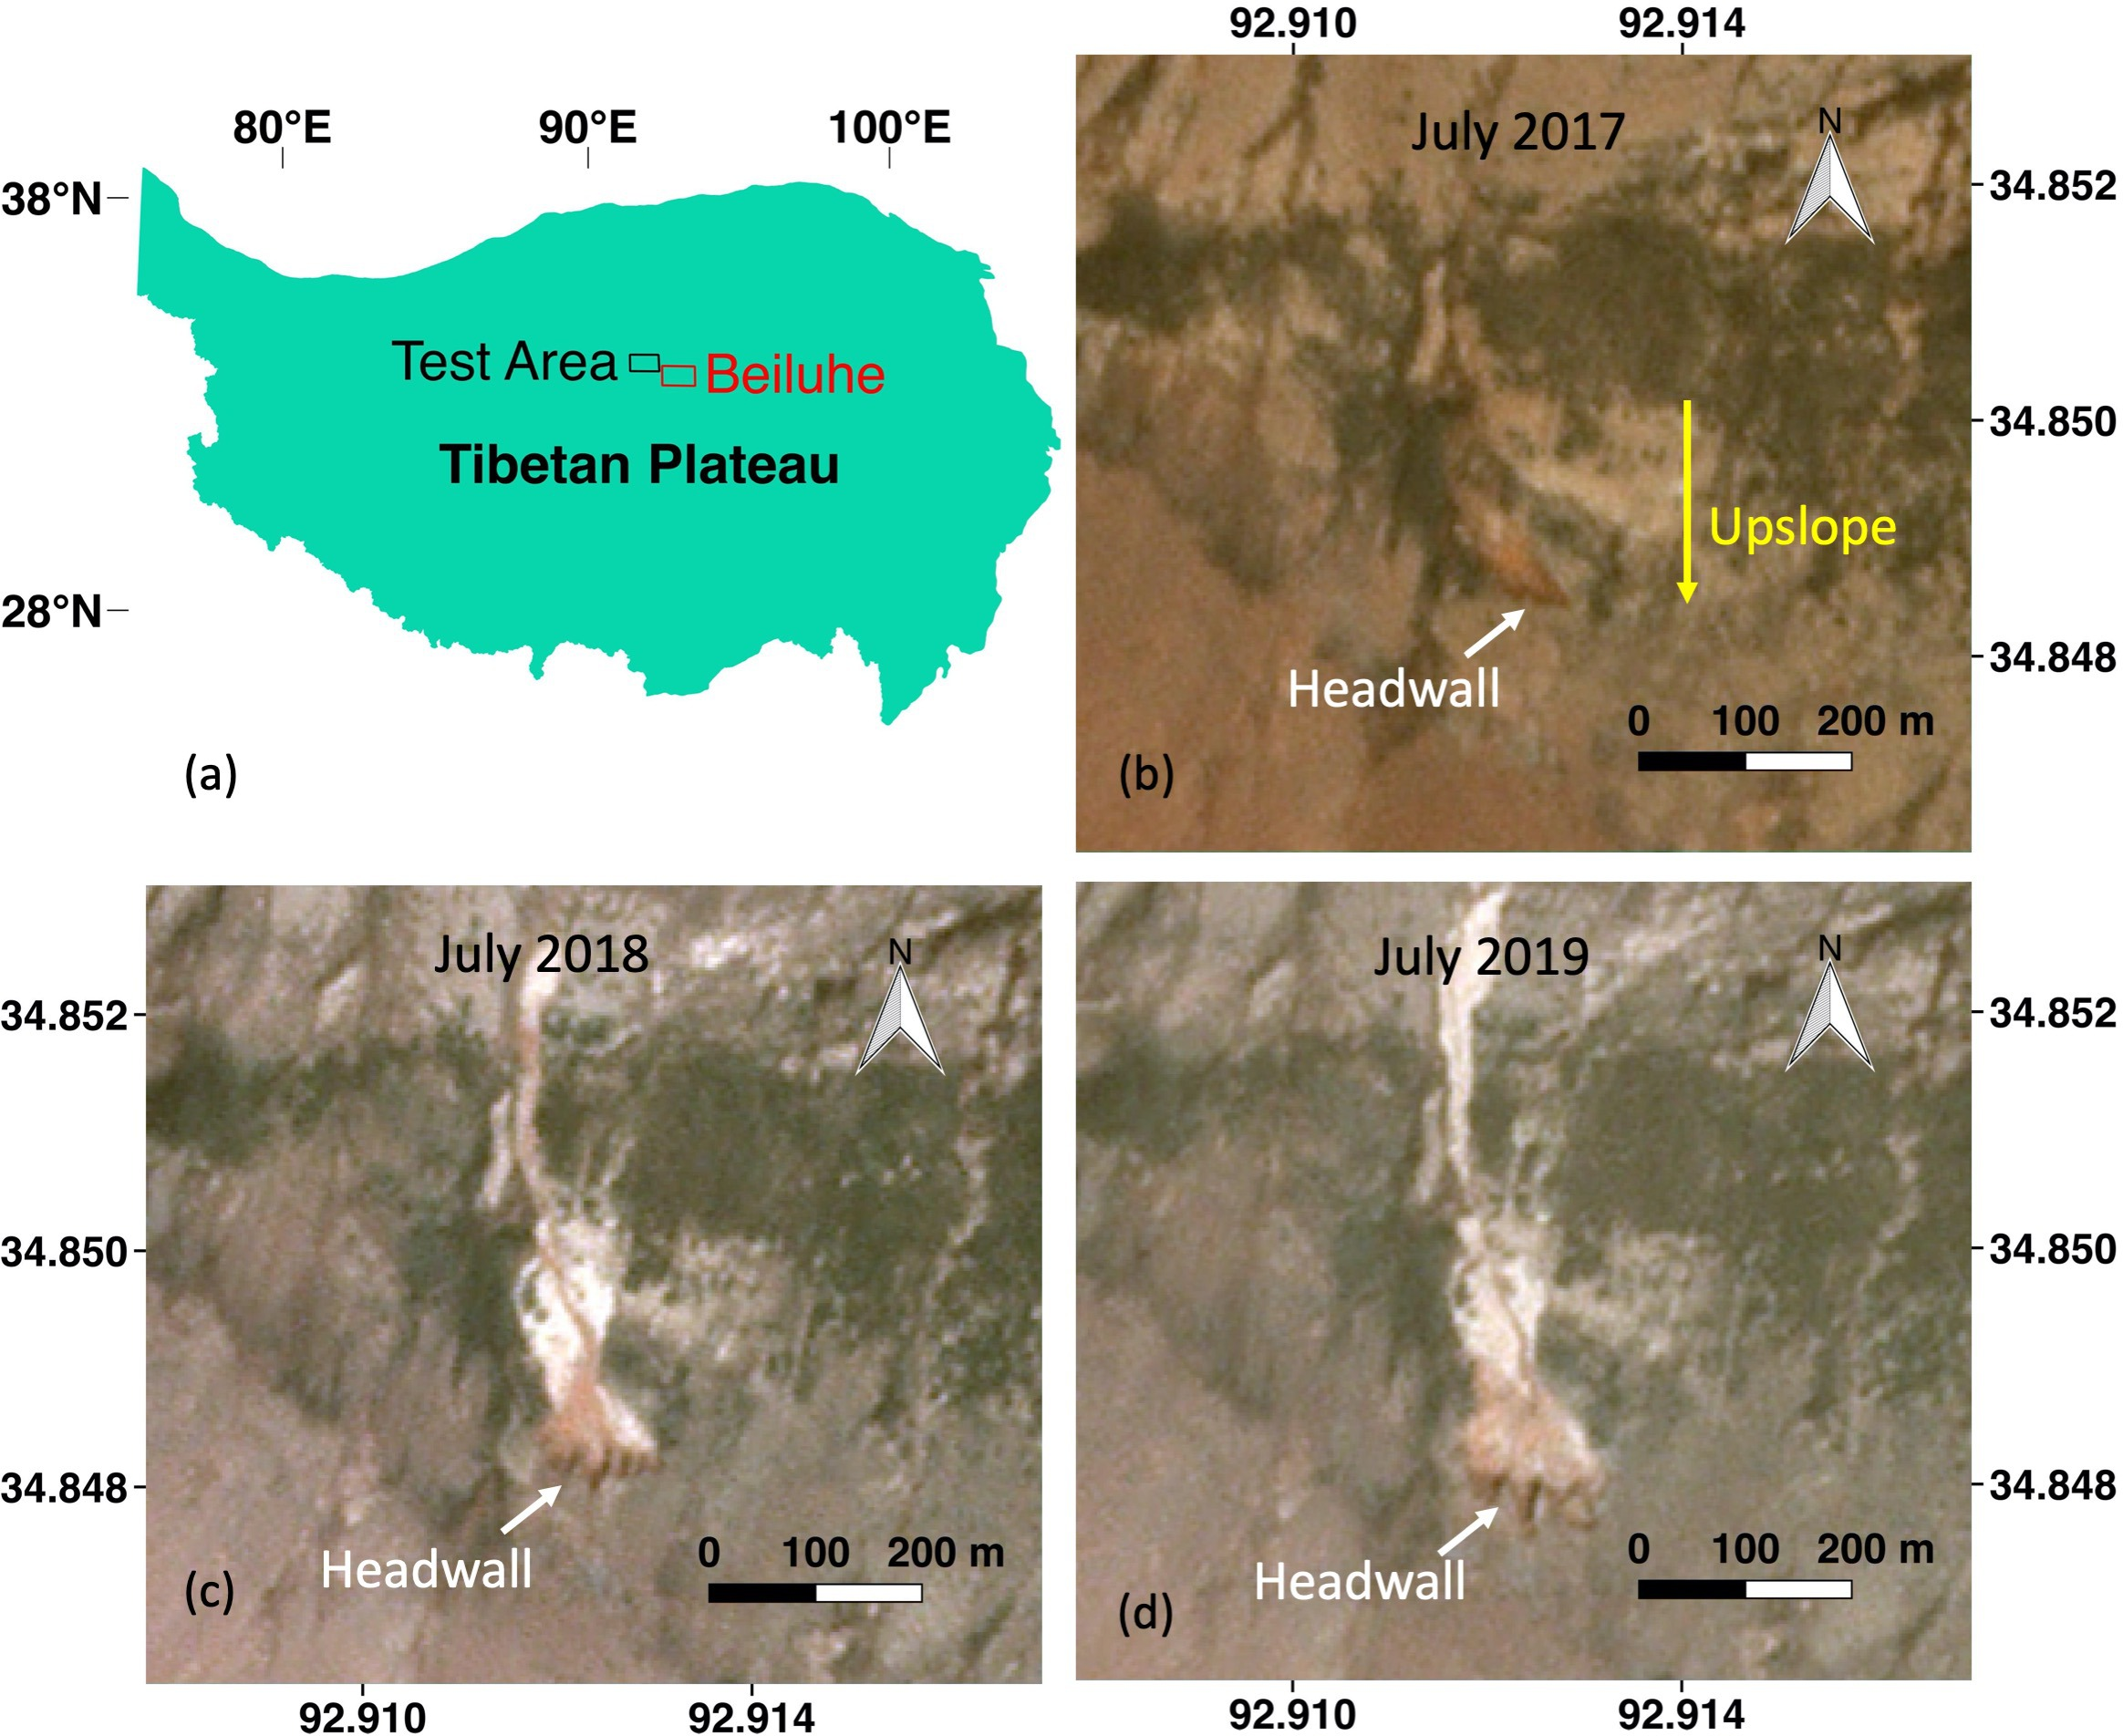
\includegraphics[width=14cm]{figs/rts_multi_images_study_area_v2_trim.jpg}
	\caption{The study area and development of a retrogressive thaw slump (RTS). The red and black rectangle in (a) shows the extent of our study area and test area on the Tibetan Plateau. (b) to (d) are Planet images (2017, 2018, and 2019) of an RTS whose central location is 92.912$^\circ$ E, 34.848$^\circ$ N. The white arrows point the position of the headwall. In (b), the yellow arrow indicates the upslope direction.}
	\label{fig_multi_rts_image_studyarea}
\end{figure}


%Data
The data include images from Planet CubeSat and RTS boundaries in July 2017, 2018, and 2019.
%address why only choose the images starting from 2017? 
We only use images after 2017 because images from Planet CubeSat constellation (Planetscope) are available after that time in our study area.  
In July, vegetation reaches its maximum coverage, and active RTSs are on the rapid stage of thawing processes. 
Therefore, identifying RTSs would be relatively easy during this period.
These images have four bands (blue, green, red, and near-infrared) with the spatial resolution of 3 m. 
Each image covers an approximate area of 10 km by 30 km.
Table \ref{table_image_list} lists the count and acquisition date of these images in from 2017 to 2019. 
Because of the variation of cloud cover and image coverage, the image count in different years are different.
The RTS boundaries are derived from manual delineation on Planet images using the same method in \cite{huang2020using}, parts of which will be used for training our automatic method. 
We consider all the RTS boundaries as ground truths in the validation step, and 70\% of them are cross-checked in the field in 2014 and 2018. %on other satellite images? 
%The steps of downloading as well as pre-processing of Planet images and collecting ground truths are presented by \cite{huang2020using}.

\begin{table}[ht]
\footnotesize
\caption{Count and acquisition date of images from the Planetscope satellites.}
\label{table_image_list}
\centering
%% \tablesize{} %% You can specify the fontsize here, e.g. \tablesize{\footnotesize}. If commented out \small will be used.
%\begin{tabular}{cc m{2.2cm}  m{2.2cm}  m{2.2cm} ccc}
\begin{tabular}{c  c  m{2.5cm}   c m{3.0cm} }
\toprule
 \multirow{2}{*}{ \textbf{Year/Month}}  & \multicolumn{2}{c}{ \textbf{Beiluhe}} &  \multicolumn{2}{c}{ \textbf{Test Area}}\\
 & Count & Acquisition date & Count & Acquisition date \\
\midrule
 2017 July & 71 & 17, 19, and 20 & 30 & 19 and 20 \\
 2018 July & 52 & 20, 24, and 25 & 31 & 15 and 16 \\
 2019 July & 46 & 25, 27, and 30 & 52 &  8, 24, 25, 27, and 30\\

\bottomrule
\end{tabular}

%\raggedright \#: the continuous experiment number
\end{table}


\section{Methods}
\label{sec_meth}

%TODO: add the whole flowchart.
% The major steps includes pre-processing of multi-temporal Planet images, training, prediction,  polygon-based change detection, and post-processing. 
%training on multi-temporal images, prediction on multi-temporal images, then polygon-based change detection: (1) removing false positives based on multi-temporal mapping results, (2) polygons based change detection based and got the expanding areas. 


\subsection{Pre-processing of multi-temporal images}
\label{sec_preprocessing}

We collected and pre-processed Planet CubeSat images before applying deep-learning-based mapping methods. 
We downloaded Planet images via Planet website (\url{www.planet.com}) via its Education and Research Program \citep{team2017planet}. 
For the images of each year, we followed the same steps presented by \cite{huang2020using} to pre-process them and obtained a mosaic covering the study area. 
%The steps of downloading, band extracting, stretching, and sharpening of these images in different years are presented by \cite{huang2020using}. 
%Co-registration
To increase the relative positional accuracy among multi-temporal images, we apply co-registration to the three mosaic images from 2017 to 2019. 
Firstly, we chose the mosaic image in \cite{huang2020using} as the reference image because it has been well pre-processed. Secondly, we used the scale-invariant feature transform algorithm \citep{lowe2004distinctive} with a GPU implement (\url{https://github.com/pitzer/SiftGPU}) to find tie-points between other mosaic images and the reference image \citep{huang2016a}. 
Lastly, we warped these images by using the Geospatial Data Abstraction Library (GDAL) with a first-order polynomial model.
%TODO: add co-registration accuracy in the supplementary files, also mentioned original 10 m accuracy 

% test histogram normalization in pre-processing steps (as noted, the histogram normalization did not improve the quanlity of Planet images, so we may just skip further steps)


\subsection{Delineating RTSs in different years}
\label{sec_delineating}

We used a deep-learning-based algorithm \citep{huang2020using} to automatically delineate RTSs on multi-temporal images.
Compared with the method in \cite{huang2020using},  the innovation of this work includes (1) training without using negative training polygons and (2) improving RTS mapping results by utilizing RTS dynamic information in multi-temporal images. 
The details will be presented as the following.

% not include negative training polygons, has bad results, but can be removed by the multi-temporal information. 

\subsubsection{Preparing training data} 
\label{sec_prepare_training}

%\subsubsection{Training a single model} 
%\label{sec_training_model}

% Preparing training data
The training data were derived from training polygons and Planet images in 2017, 2018, and 2019. 
We considered all the ground truths as positive training polygons but did not include any negative training polygons. 
Negative training polygons are necessary for distinguish land cover that are similar to RTSs but need ground information or some initial tests to generate them. 
However, generating negative training polygons will be impractical for mapping RTSs in a large area. 
Without negative training polygons, the mapping results may contain a lot of false positives, but we can utilize the RTS dynamic information in multi-temporal images to remove them (see section \ref{sec_improving_using_rts_dynamic}).
For the training polygons and Planet images in each year, we extracted sub-images with a buffer area of 300 m. 
Then we subdivided all sub-images into patches by setting a patch size as 480 pixels with an overlap of 160 pixels. 
Details of the extracting and subdividing operation are presented by \cite{huang2018automatic}.
To improve the volume of training data and generalization of the trained model, we applied data augmentation (flipping, blurring, cropping, and scaling) to the patches. 
Lastly, we merged all the patches from different years to a single training dataset. 


\subsubsection{Training a single model and predicting RTSs in different years}
\label{sec_train_prediction}

% training
We trained a deep-learning model, i.e., DeepLabv3+ \citep{chen2018encoder-decoder}, by using the training data derived in section \ref{sec_prepare_training}. 
\cite{huang2020using} have proofed that a well-trained DeepLabv3+ can delineate RTSs and obtain their boundaries that are very close to manual delineation. 
In this study, instead of training different models for different years, we only trained a single model because DeepLabv3+ has a high capability to represent RTS features in multi-temporal images, more importantly, a generic model can save a lot of computing resources, especially when expanding the time domain.
We used the same hyper-parameter presented in \cite{huang2020using} to train this model. 
To evaluate the robustness of the model, we utilized k-fold cross-validation (k=3, 5, and 10)  as commonly used in machine learning. 
 %TODO: How about the test Area? use which trained model?
%k-fold cross-validation. 

% prediction
We used the trained model to predict RTSs on in 2017, 2018, and 2019 mosaic images. 
The steps of predicting RTSs in one year include (1) dividing it to numerous small patches, (2) predicting RTS or non-RTS pixels, (3) mosaicked the binary patches using GDAL and obtained a binary mosaic, (4) polygonizing the binary mosaic, and (5) removing polygons smaller than 0.3 ha. 
The size and overlap of each patches for prediction is the same to the one for preparing training data (section \ref{sec_prepare_training}). 
To improve efficiency, we adopted a parallel strategy to predict RTSs in different years.


\subsubsection{Improving RTS mapping results using the RTS dynamic feature}
\label{sec_improving_using_rts_dynamic}

Many mapped polygons were erroneously identified as RTS polygons can be removed by utilizing the RTS dynamic feature. 
As shown in Fig. \ref{fig_rts_expanding}, an active RTS can expand toward upslope annually, even for a non-active RTS, its extent cannot shrink. 
Therefore, we can use this dynamic feature to remove non-RTS mapped polygons. 
Firstly, we obtained a union (Fig. \ref{fig_rts_expanding}) of mapped polygons at the same location.
The steps of obtaining the union include (1) choosing a mapped polygon as initial union, (2) scanning through all mapped polygons until find a mapped polygon that still available (not merged to other unions) and overlap the union, (3) merging the found mapped polygon to union and updating the union, and (4) repeating steps (2) and (3) until cannot find a new mapped polygon can be merged to the union. 
Secondly, we calculated the intersection over union (IOU) for mapped polygons in each year (termed as ``time-IOU") as follows, 
\begin{equation}
IOU(A,B)_{year}=area(A \cap B)/area(A \cup B)
\label{equ_time_iou}
\end{equation}
where \emph{A} is a mapped polygon in the specific year and \emph{B} is the union. 
Due to the dynamic of RTSs, the time-IOU of an active RTS will monotonically increase over time. 
If the RTS is already stabilized, its time-IOU will remain the same over time. 
In consideration of the delineation error (e.g., the RTS boundaries in different years at non-headwall parts are not exactly overlap each other as shown in Figs. \ref{fig_rts_expanding} and \ref{fig_rts_change_det}), a threshold of $-0.1$ was set to determine the time-IOU of an RTS is monotonically increasing, that is, if all the differences ($IOU_{next\_year}-IOU_{year}$) are greater than $-0.1$, we consider the time-IOU is monotonically increasing. 
Thirdly, in the Beiluhe region, almost all the RTSs were initiated in or before 2016 \citep{luo2019recent}.
Therefore, we can assume that at a specific location where an RTS emerges, it presents three mapped polygons and each in 2017, 2018, and 2019. 
Lastly, we removed mapped polygons in a location that do not satisfy the three-polygon assumption or the time-IOU is not monotonically increasing.
 
%[ht]
\begin{figure} 
	\centering
	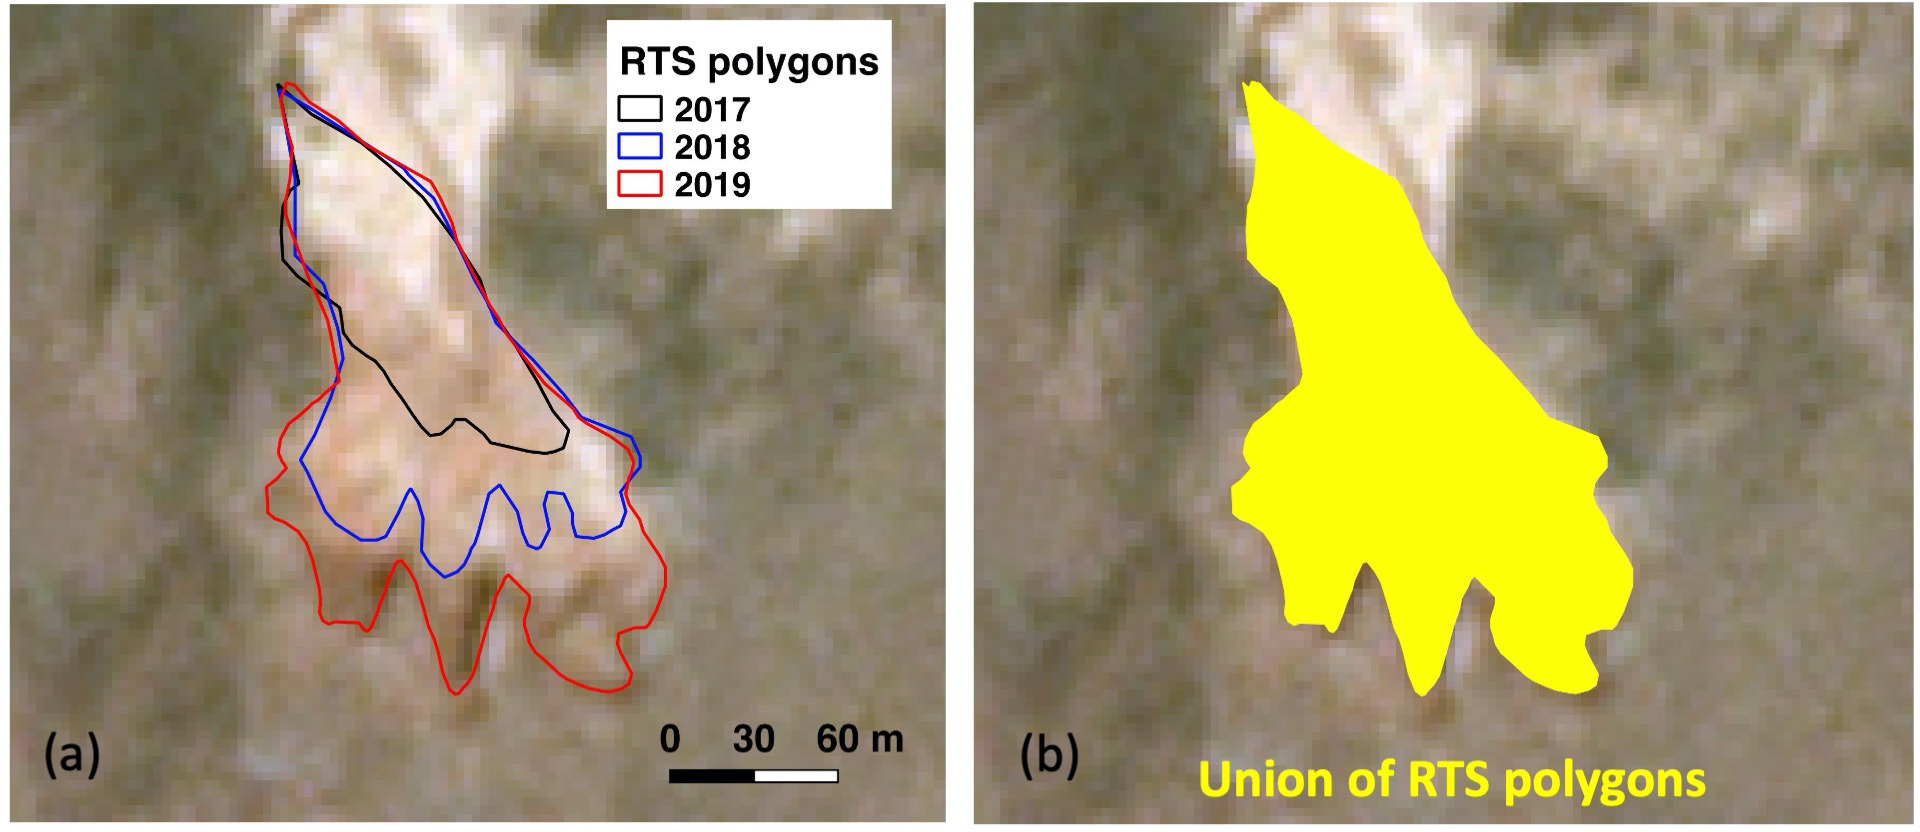
\includegraphics[width=14cm]{figs/rts_expanding_example_trim}
	\caption{RTS polygons (a) representing their boundaries from 2017 to 2019 and the union (b) of these polygons. The background is 2019 Planet images, and the RTS is the same to the one shown in Fig. \ref{fig_multi_rts_image_studyarea}}
	\label{fig_rts_expanding}
\end{figure}


\subsubsection{Validating mapped polygons}
\label{sec_validate_mapped_polygons}

To validate mapped polygons, we calculate F1 scores \citep{huang2020using} for mapped polygons in each year separately. 
For each  year, we calculate IOU values between mapped polygons and the corresponding ground truths. 
We set a threshold of 0.5 to decide a mapped polygon is a false positive or true positive.
After obtaining the count of true positives, false positives, and false negatives, we can calculate the precision and recall, then calculate the F1 score using the following euqation. 
\begin{equation}
F1=2 \times Precision \times Recall / (Precision + Recall)
\label{equ_f1score}
\end{equation}
More details of the F1 score and its implication can be found in \cite{huang2020using}.
We repeated the calculation of F1 scores for different years and obtained the corresponding values. 

To assess the performance of the delineating method in this paper, we calculated the average precision (AP) values for mapping results in different years, then averaged them. 
AP values are based on precision-recall curves which is an effective metric for evaluating the algorithm performance \citep{huang2020using}.
A higher average of AP values indicates the better performance of the method. 

\subsection{Detecting changes of RTS boundaries}
\label{sec_detect_rts_changes}

This study will provide a method to automatically detect changes of RTS boundaries and calculate their annual retreat distance.
The RTS boundaries are in vector format and can be derived from manual delineation or automatic mapping. 
The main steps include polygon-based change detection, removing false changes, and calculating retreat distance as follows, 

\subsubsection{Polygon-based change detection}
\label{sec_polygon_change_det}

To obtain the annual RTS changes, we conducted change detection for RTS boundaries between this year and the previous year, that is, comparing 2017 with 2018 and 2018 with 2019. 
 As shown in equation \ref{equ_polygon_diff}, for a specific location has mapped polygons in different years, a polygon in year \emph{t} minus the one in year \emph{t-1} can result in an expanding polygon or multiPolygon. 
We used the ``difference'' function in Shapely (\url{https://pypi.org/project/Shapely}) to implement the subtraction in equation \ref{equ_polygon_diff}.
\begin{equation}
E= P_{t} - P_{t-1}
\label{equ_polygon_diff}
\end{equation}
where \emph{P} is an RTS polygon, \emph{t} represents year, and \emph{E} is the expanding polygon or multiPolygon. 
While $P_{t} - P_{t+1}$ can result in a shirking polygon, but it does not correspond to the dynamic feature of an RTS; instead, it is a result of delineation errors. 
Fig. \ref{fig_rts_change_det} shows an example of the subtraction operation between the RTS boundaries in 2017 and 2018. 
%removing the narrow parts. 
With the consideration of delineation errors and the resolution (3 m) of Planet images, we removed the narrow parts of expanding multiPolygons using buffer operation as follows, 
\begin{equation}
P_{non\text{-}narrow}= P.\text{buffer}(-r).\text{buffer}(r*f) \cap P
\label{equ_polygon_buffer}
\end{equation}
where \emph{P} is a polygon or multiPolygon, \emph{r} is the value of buffer operation,  \emph{f} is a factor between 1 to 2 for avoiding uncertainties of buffer operation. 
%TODO: check or update the r and f value in the codes
In this study, we set \emph{r} as 3 and \emph{f} as 1.6 after initial experiments and used ``buffer'' function in Shapely.
To make it practical for calculating polygon attributes (e.g., area and parameter) and removing false changes (section \ref{sec_removing_false_change}), we converted all the multiPolygons to Polygons.

%a figure showing a multiPolygon and its narrow parts. 
%[ht]
\begin{figure} 
	\centering
	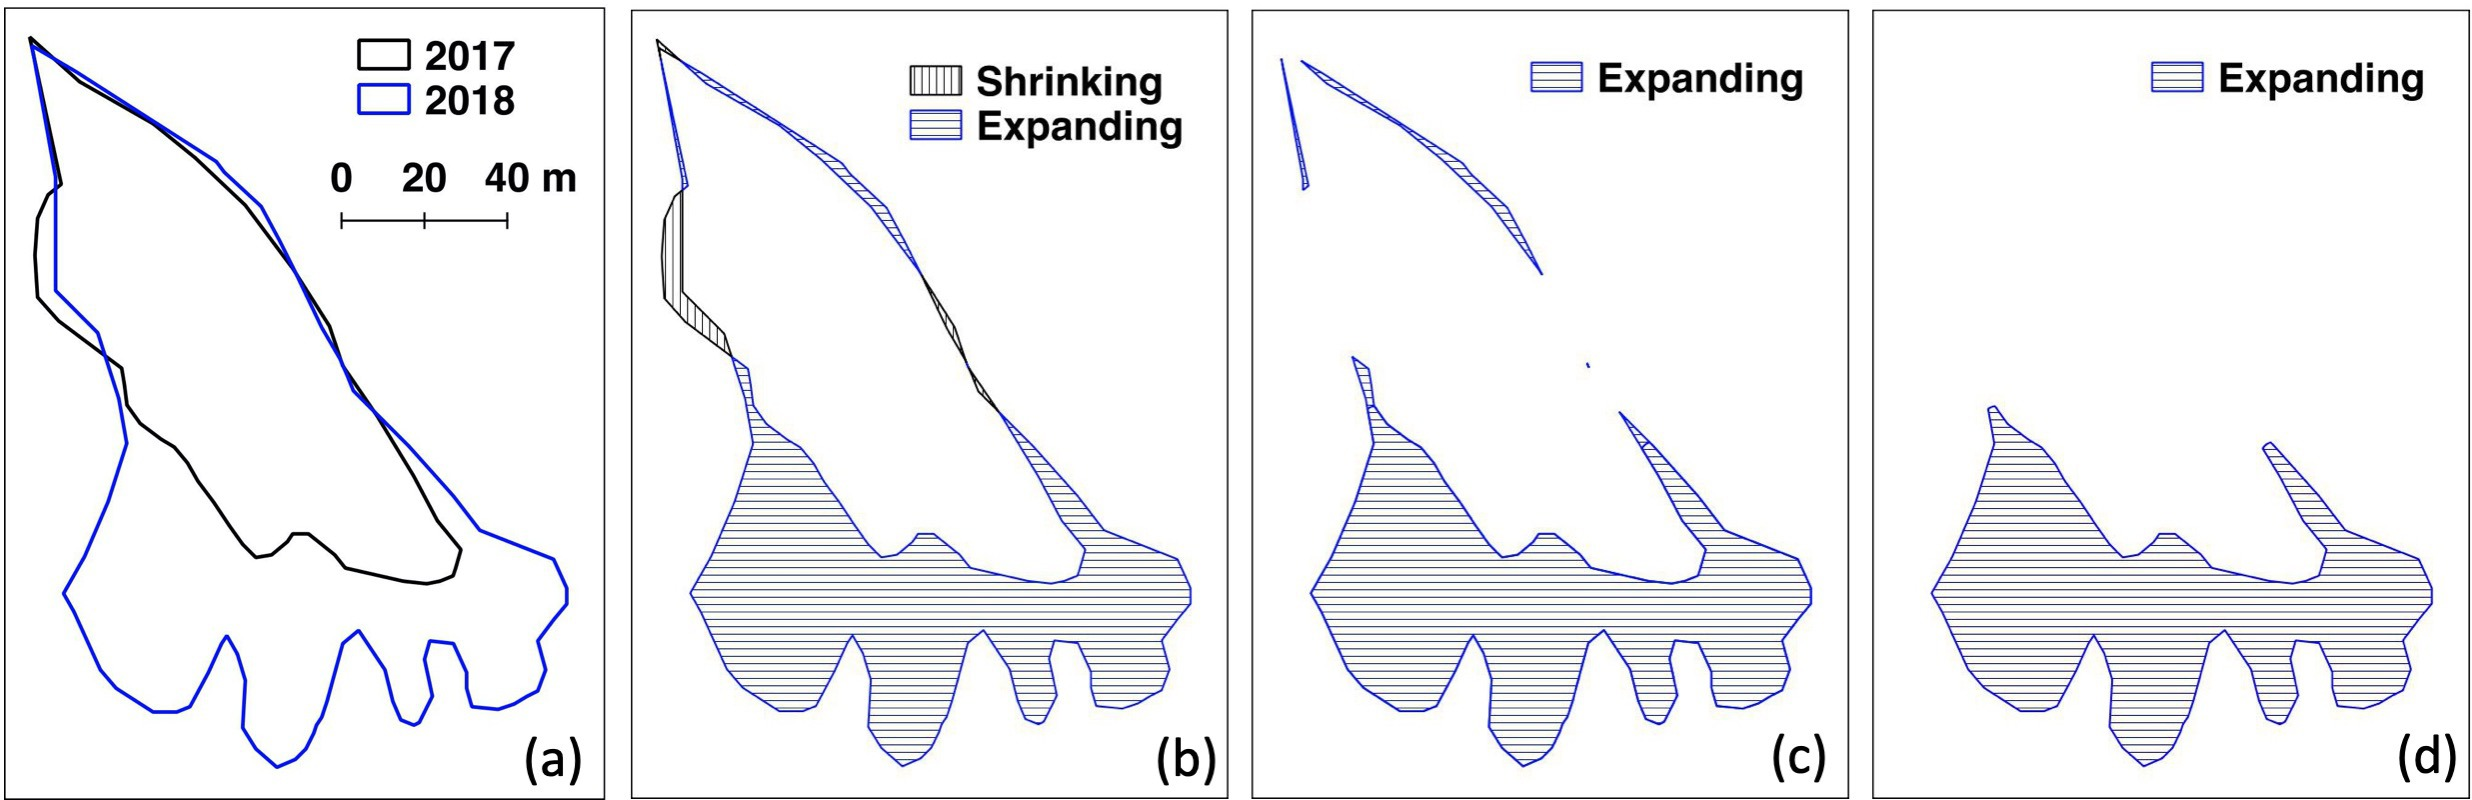
\includegraphics[width=14cm]{figs/rts_polygon_change_det_trim}
	\caption{An example of the polygon-based change detection. (a) shows the boundaries of an RTS (Fig. \ref{fig_rts_expanding}a) in 2017 and 2018. $P_{2018}-P_{2017}$ results in an expanding multiPolygon (b) and the corresponding non-narrow parts (c). $P_{2017}-P_{2018}$ results in a shrinking multiPolygon (d).}
	\label{fig_rts_change_det}
\end{figure}

%a multi-polygon to polygons and calculate the attributes: area, circularity, 
%zeroIntersection, two or more intersections, holes, relative elevation, retreat distance. 

\subsubsection{Removing false changes}
\label{sec_removing_false_change}

%Polygon change detection. \\\\


\subsubsection{Calculating retreat distance}
\label{sec_cal_retreat_dis}

%Calculating the retreat distance. \\\\


\subsubsection{Validating RTS changes}
\label{sec_validation_change}



\section{Results}
\label{sec_result}

\subsection{The performance of mapping task using multi-temporal images}
\label{sec_mapping_performance}

Improvement by applying time IOU and occurrence


\subsection{RTSs expansion from 2017 to 2019}
\label{sec_rst_expanding}

Retreat distance. 


\section{Discussion}
\label{sec_discussion}

good

A new emergence RTS was missed. 

\section{Conclusions}
\label{sec_conclusion}

 good

\section{Data and codes}
\label{sec_data_codes}

Planet images can be downloaded via. 
Codes are available on GitHub (\url{https://github.com/yghlc/ChangeDet_DL}) after the acceptance of this paper.

\section{Acknowledgments}
\label{sec_acknowledgments}

Thanks to ...


%% The Appendices part is started with the command \appendix;
%% appendix sections are then done as normal sections
%% \appendix

%% \section{}
%% \label{}

\section{References}
\label{sec_reference}

%% If you have bibdatabase file and want bibtex to generate the
%% bibitems, please use
%%
\bibliographystyle{elsarticle-harv} 
%\bibliography{poygon_based_rts_changeDet.bib}
% the bib file in "~/codes/Texpad/shared_files"
\bibliography{permafrost_rs_ref.bib}

%% else use the following coding to input the bibitems directly in the
%% TeX file.

%\begin{thebibliography}{00}
%
%%% \bibitem[Author(year)]{label}
%%% Text of bibliographic item
%
%\bibitem[ ()]{}
%\end{thebibliography}


\end{document}

\endinput
%%
%% End of file `elsarticle-template-harv.tex'.
